
\documentclass{beamer}

\usetheme{Warsaw}
\setbeamercovered{transparent}

\usepackage[german]{babel}
\usepackage[latin1]{inputenc} \usepackage{mathptmx,amsmath}
\usepackage[T1]{fontenc}

\title[Beamer-Paket]{Pr\"asentationen mit dem Paket \glqq Beamer \grqq}
\subtitle{Beispielsfoliensatz}

\author[Autor]{Name des Autors}
\institute[inst]{Name des Institutes}
\date{\today}

\AtBeginSubsection[]
{
    \begin{frame}<beamer>{Gliederung}
        \tableofcontents[currentsection,currentsubsection]
    \end{frame}
}

\begin{document}

\begin{frame}
    \titlepage
\end{frame}

\begin{frame}{Gliederung}
    \tableofcontents
\end{frame}

\section{Einf\"uhrung}
\subsection[Philosophie]{Die Philosophie des Paketes}

\begin{frame}[fragile=singleslide]{Grunds\"atzliche Eigenschaften}
    \begin{itemize}
        \item Die Strukturierung erfolgt mit den \"ublichen Kommandos \verb+\section+, \verb+\subsection+, \ldots
        \item Die Aufz\"ahlungsumgebungen sind vorhanden, haben aber eine andere Optik
        \item Prinzipiell sind alle \LaTeX-M\"oglichkeiten verwendbar, z.B. Formelsatz
            \begin{equation}
                \det\begin{pmatrix}2&\alpha\\1&2\end{pmatrix} = 4-\alpha.
            \end{equation}
        \item Das Layout wird durch Stilvorlagen (\alert{Themes}) festgelegt
        \item Druckversionen einer Pr\"asentation lassen sich leicht erstellen
        \item Dynamische Pr\"asentationseffekte werden unterst\"utzt
    \end{itemize}
\end{frame}


\begin{frame}{Overlays (\"Uberlagerte Folien in Folge)}
    eine Folienfolge mit \"Uberlagerung kann erzeug werden
    \begin{itemize}
    \item mit dem \texttt{pause}-Befehl:
        \begin{itemize}
        \item Erster Punkt \textsl{(sichtbar von Anfang an)}.
        \pause
        \item Zweiter Punkt \textsl{(sichtbar ab Folie 2)}.
        \end{itemize}
    \item mittels Overlay-Spezifikationen:
        \begin{itemize}
        \item<3-> Erster Punkt \textsl{(sichtbar ab Folie 3)}.
        \item<4-> Zweiter Punkt \textsl{(sichtbar ab Folie 4)}.
        \end{itemize}
    \item mit dem allgemeinen \texttt{uncover}-Befehl:
        \begin{itemize}
        \uncover<5->{\item Erster Punkt \textsl{(sichtbar ab Folie 5)}.}
        \uncover<6->{\item Zweiter Punkt \textsl{(sichtbar ab Folie 6)}.}
        \end{itemize}
    \end{itemize}
\end{frame}

\subsection{Elemente einer Pr\"asentation}
\begin{frame}{Listen}
    \begin{itemize}
    \item Aufz\"ahlung mit \texttt{itemize}.
    \item Spiegelstriche sind optisch hervorgehoben.
    \end{itemize}

    \begin{enumerate}
    \item Aufz\"ahlungen mit \texttt{enumerate}.
    \item Zahlen sind optisch hervorgehoben.
    \end{enumerate}

    \begin{description}
    \item[Erster Punkt] Aufz\"ahlungen mit \texttt{description}.
    \item[Zweiter Punkt] Der Parameter der Einzelpunkte ist farblich hervorgehoben und der weitere Text ist stark eingedr\"uckt.
    \end{description}

\end{frame}

\begin{frame}{Gerahmte Texte}
    \begin{block}{}
        Dieser Text erscheint gerahmt (sofern dies vom Layout-Thema unterst\"utzt wird).
    \end{block}
    \begin{block}{Rahmen\"uberschrift}
        Dieser Text erscheint gerahmt.
    \end{block}
    \alert{Hervorhebung} mit dem \texttt{alert}-Befehlt oder:
    \begin{alertblock}{Farblich hervorgehobener Rahmen}
        Dieser Text erscheint gerahmt und hervorgehoben.
    \end{alertblock}
    \begin{exampleblock}{Beispiel (andere Farbe)}
        Dieser Text wird als Beispiel angesehen.
    \end{exampleblock}
\end{frame}

\begin{frame}{Mehrspaltige Texte}
    \transdissolve
    \begin{columns}
        \begin{column}{5cm}
            \begin{itemize}
            \item Die Umgebung \texttt{columns} erlaubt die Erzeugung mehrerer Spalten.
            \item<2-> Jede Spalte wird durch die Umgebung \texttt{column} erzeugt, die als Parameter die Spaltenbreite enh\"alt.
            \item<2-> Die Ausrichtung der Spalten wird \"uber Optionen geregelt.
            \end{itemize}
        \end{column}
        \begin{column}{5cm}
            \visible<2-> {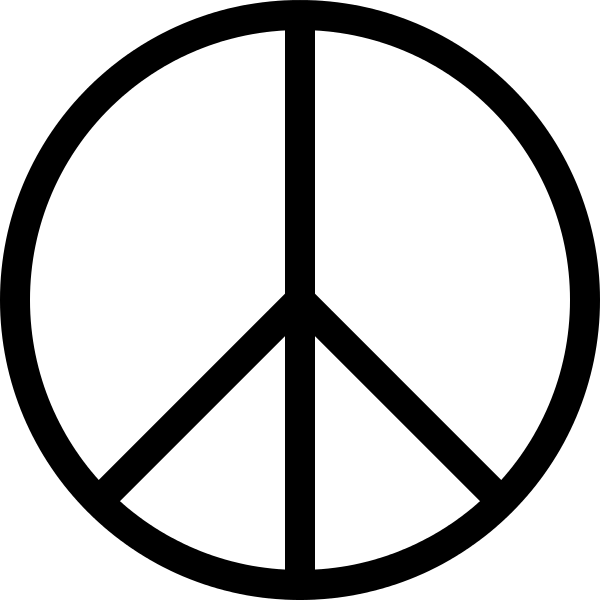
\includegraphics[clip,width=5cm]{give_peace_a_chance}}
        \end{column}
    \end{columns}
\end{frame}


\end{document}



